\documentclass[12pt,a4paper]{article}

% ── Packages ──────────────────────────────────────────────────────────────────
\usepackage{fontspec}
\usepackage[margin=2.5cm]{geometry}
\usepackage{graphicx}
\usepackage{booktabs}
\usepackage{longtable}
\usepackage{array}
\usepackage{xcolor}
\usepackage{hyperref}
\usepackage{amsmath}
\usepackage{amssymb}
\usepackage{float}
\usepackage{caption}
\usepackage{subcaption}
\usepackage{titlesec}
\usepackage{fancyhdr}
\usepackage{parskip}
\usepackage{microtype}
\usepackage{enumitem}
\usepackage{tcolorbox}
\usepackage{tabularx}
\usepackage{multirow}
\usepackage{setspace}

% ── Fonts ──────────────────────────────────────────────────────────────────────
\setmainfont{Latin Modern Roman}
\setsansfont{Latin Modern Sans}
\setmonofont{Latin Modern Mono}

% ── Colours ───────────────────────────────────────────────────────────────────
\definecolor{navy}{RGB}{14,40,65}
\definecolor{sblue}{RGB}{21,96,130}
\definecolor{sorange}{RGB}{233,113,50}
\definecolor{sgreen}{RGB}{25,107,36}
\definecolor{lgrey}{RGB}{232,232,232}
\definecolor{darktext}{RGB}{30,41,59}

% ── Section styling ───────────────────────────────────────────────────────────
\titleformat{\section}{\large\bfseries\color{navy}}{\thesection}{1em}{}[\color{sblue}\titlerule]
\titleformat{\subsection}{\normalsize\bfseries\color{sblue}}{\thesubsection}{1em}{}
\titleformat{\subsubsection}{\normalsize\itshape\color{darktext}}{\thesubsubsection}{1em}{}

% ── Header/footer ─────────────────────────────────────────────────────────────
\pagestyle{fancy}
\fancyhf{}
\fancyhead[L]{\small\textcolor{sblue}{Agentic SABRE}}
\fancyhead[R]{\small\textcolor{sblue}{Technical Report — April 2026}}
\fancyfoot[C]{\thepage}
\renewcommand{\headrulewidth}{0.4pt}

% ── Hyperref ──────────────────────────────────────────────────────────────────
\hypersetup{
  colorlinks=true, linkcolor=sblue, citecolor=sblue, urlcolor=sblue,
  pdftitle={Agentic SABRE Technical Report},
  pdfauthor={Henry Kabuye}
}

% ── tcolorbox styles ──────────────────────────────────────────────────────────
\tcbset{
  keybox/.style={colback=lgrey!60, colframe=sblue!60, fonttitle=\bfseries\small,
                 left=4pt, right=4pt, top=3pt, bottom=3pt, boxrule=0.5pt},
  notebox/.style={colback=sorange!10, colframe=sorange!60, fonttitle=\bfseries\small,
                  left=4pt, right=4pt, top=3pt, bottom=3pt, boxrule=0.5pt}
}

% ── Misc ──────────────────────────────────────────────────────────────────────
\setlength{\parskip}{6pt}
\captionsetup{font=small, labelfont={bf,color=sblue}}
\graphicspath{{../Figures/}}

% ══════════════════════════════════════════════════════════════════════════════
\begin{document}

% ── Title page ────────────────────────────────────────────────────────────────
\begin{titlepage}
  \centering
  \vspace*{1.5cm}
  {\Huge\bfseries\color{navy} Agentic SABRE\par}
  \vspace{0.6cm}
  {\large\color{sblue}
    An Uncertainty-Aware Multi-Agent Framework\\
    for Adaptive Ransomware Detection\par}
  \vspace{1.2cm}
  \rule{\textwidth}{1.5pt}
  \vspace{0.8cm}
  {\large Henry Kabuye\\
  PhD Student, Northumbria University\par}
  \vspace{0.4cm}
  {\normalsize
    Principal Supervisor: Dr Biju Issac\\
    Secondary Supervisor: Dr Neera Jeyamohan\par}
  \vspace{0.8cm}
  {\normalsize Technical Report — April 2026\par}
  \vspace{1.5cm}
  \rule{\textwidth}{1.5pt}
  \vspace{1.0cm}
  \begin{tcolorbox}[keybox, title=Abstract]
    \small
    Ransomware detection demands evidence from multiple modalities — static PE
    structure, runtime hypervisor telemetry, and threat-intelligence discourse — yet
    no single detector dominates across all sample types. SABRE addresses this through
    a three-agent architecture: a \textbf{Semantic CNN} (RDset, 138,047 PE samples), a
    \textbf{Behavioural CNN} (RanSMAP, 751,588 hypervisor telemetry windows), and a
    \textbf{Knowledge CNN} (RansKnow, 200 MITRE ATT\&CK samples). Each agent produces
    a probability and an uncertainty estimate via Monte Carlo Dropout. A \textbf{Decision
    MLP} fuses the six-dimensional score vector
    $[\hat{p}_{\text{sem}},\hat{p}_{\text{beh}},\hat{p}_{\text{know}},
      \sigma_{\text{sem}},\sigma_{\text{beh}},\sigma_{\text{know}}]$
    (augmented with CTGAN and calibrated with temperature scaling) into a fused risk
    $\hat{p}$. An \textbf{uncertainty-aware triage policy}, tuned by Bayesian
    optimisation (TPE), maps $(\hat{p}, \sigma_{\max})$ to
    \textsc{auto-contain} / \textsc{escalate} / \textsc{allow}. Two new
    mechanisms extend the baseline: \textbf{per-agent peer consultation}
    ($\kappa_{\text{local}}$) adjusts uncertain agent scores before fusion, and an
    \textbf{expert feedback loop} enables analyst corrections to drive incremental MLP
    retraining. The fused system achieves \textbf{97.2\% balanced accuracy, 100\% TPR,
    94.7\% precision, and zero false negatives} on a 4,000-sample evaluation.
  \end{tcolorbox}
\end{titlepage}

\tableofcontents
\newpage

% ══════════════════════════════════════════════════════════════════════════════
\section{Introduction}
\label{sec:intro}

Ransomware remains one of the most operationally damaging classes of malware.
Its continued evolution through polymorphism, living-off-the-land techniques, and
behavioural obfuscation means that signature-based defences are insufficient. Modern
detectors must adapt to out-of-distribution samples, handle evidence of varying quality,
and support human-in-the-loop oversight.

Three challenges motivate the SABRE design:

\begin{enumerate}[leftmargin=2em]
  \item \textbf{Heterogeneous evidence.} Static PE features, runtime storage and memory
    telemetry, and threat-intelligence discourse encode distinct aspects of ransomware
    behaviour. No single modality dominates across all sample types.

  \item \textbf{Missing uncertainty signals.} Standard ML classifiers produce point
    predictions. An aggressive threshold creates false positives and operational
    disruption; a conservative one misses threats. Out-of-distribution samples make
    confidence values unreliable without explicit uncertainty quantification.

  \item \textbf{Operational tractability.} A deployed triage system must support
    automated containment of high-confidence threats, analyst escalation for ambiguous
    cases, and a mechanism for analyst corrections to improve the system over time.
\end{enumerate}

SABRE answers all three through a three-agent fusion pipeline with
uncertainty-aware decision making, per-agent peer consultation, and an expert
feedback loop.

% ══════════════════════════════════════════════════════════════════════════════
\section{Datasets}
\label{sec:data}

\subsection{RDset — Semantic Agent}

RDset contains \textbf{138,047 PE (Portable Executable) samples} (96,724 ransomware,
41,323 benign) with 57 structured static attributes per sample. Attributes covering
import tables, section characteristics, header metadata, and byte-level statistics are
encoded into text strings and embedded with a 384-dimensional BERT-style encoder,
producing the input feature vectors for the Semantic CNN. Training uses a
SMOTE-balanced split.

\subsection{RanSMAP / RanSAP — Behavioural Agent}

The behavioural dataset contains \textbf{751,588 hypervisor-level telemetry windows}
(750,329 ransomware, 1,259 benign — a 596:1 class imbalance). Each window comprises
16 sliding-window statistics derived from storage I/O and memory access traces:

\begin{itemize}[leftmargin=2em]
  \item Storage: average read/write throughput, read/write LBA variance, write entropy
  \item Memory: read/write/execute GPA variance; read/write/readwrite entropy; access counts
\end{itemize}

Features are normalised with a \texttt{StandardScaler} (critical for CNN performance;
without it balanced-eval AUC degrades from 0.996 to 0.621). For training, the majority
class is undersampled to 10,000 before SMOTE is applied to balance the classes.

\subsection{RansKnow — Knowledge Agent}

RansKnow comprises \textbf{200 labelled samples} derived from YouTube ransomware
practitioner discourse. Each sample is represented as a 23-dimensional feature vector
covering MITRE ATT\&CK tactic mentions (Initial Access, Execution, Persistence,
Privilege Escalation, Credential Access, Lateral Movement, Discovery, C\&C,
Exfiltration, Impact), tool mentions (Cobalt Strike, Mimikatz, PsExec, Rclone,
MegaNZ, AnyDesk, TeamViewer, BloodHound), platform signals (Windows, Linux, ESXi),
and aggregated tactic/tool counts.

% ══════════════════════════════════════════════════════════════════════════════
\section{System Architecture}
\label{sec:arch}

Figure~\ref{fig:arch} shows the full pipeline. The system is organised into five
conceptual stages: base detection, score pooling, decision fusion,
triage policy, and the expert feedback loop.

\begin{figure}[H]
  \centering
  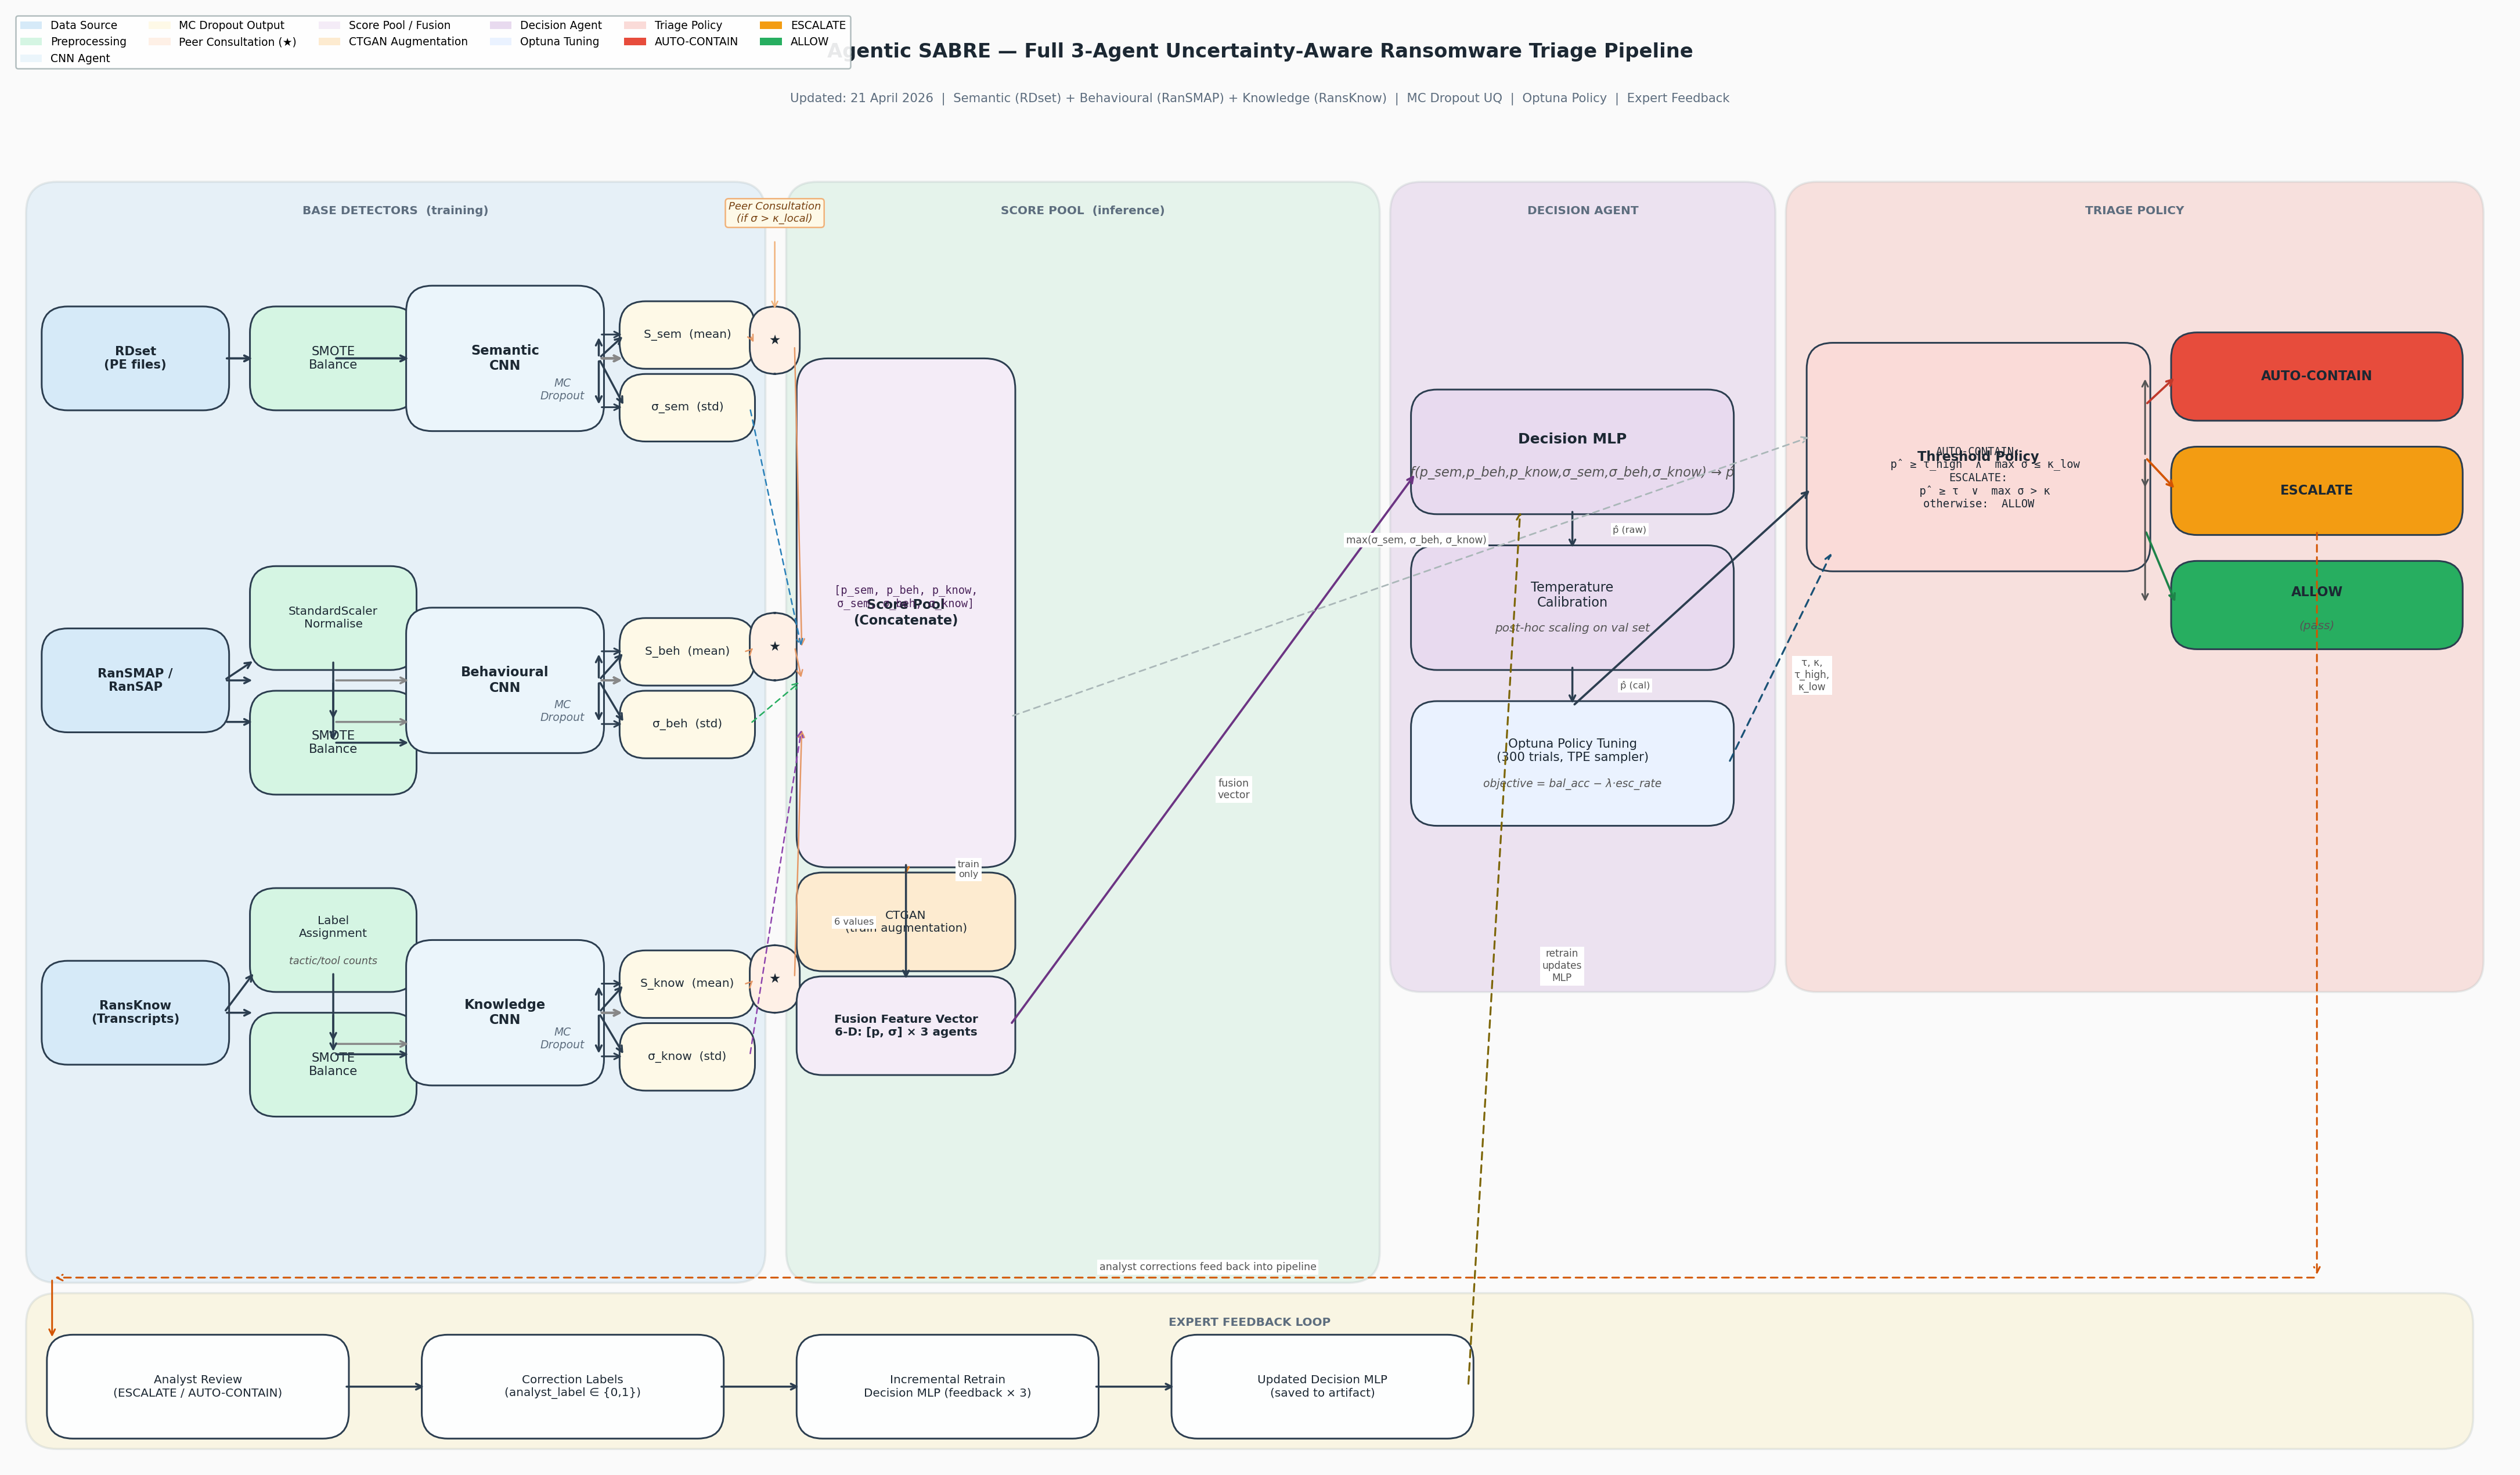
\includegraphics[width=\textwidth]{Prop_Agentic_Sabre_21_04_2026_3Agents_FullPipeline.png}
  \caption{Full Agentic SABRE pipeline. Peer consultation gates ($\bigstar$) fire per
    agent when $\sigma_{\text{agent}} > \kappa_{\text{local}}$, adjusting the
    probability before it enters the Score Pool. The Expert Feedback Loop (bottom) routes
    analyst corrections back into incremental MLP retraining.}
  \label{fig:arch}
\end{figure}

\subsection{Base Detectors}

All three agents share a common structure:

\begin{enumerate}[leftmargin=2em]
  \item A CNN classifier trained on the agent's dataset (with SMOTE balancing and, for
    the behavioural agent, StandardScaler normalisation).
  \item \textbf{Monte Carlo Dropout} uncertainty quantification at inference: the model
    is run $T$ times with dropout active; the mean output is the probability $\hat{p}$
    and the standard deviation is the uncertainty $\sigma$. The number of passes $T$ is
    adaptive — sampling continues until $\sigma$ converges (maximum $T=50$).
\end{enumerate}

\subsection{Score Pool and Decision MLP}

The six outputs $[\hat{p}_{\text{sem}}, \hat{p}_{\text{beh}}, \hat{p}_{\text{know}},
\sigma_{\text{sem}}, \sigma_{\text{beh}}, \sigma_{\text{know}}]$ are concatenated into
a \textbf{Fusion Feature Vector}. During training, CTGAN generates synthetic score-space
samples to augment the training distribution. The \textbf{Decision MLP}
$f: \mathbb{R}^6 \rightarrow [0,1]$ maps this vector to a fused risk $\hat{p}$.
Post-training \textbf{temperature scaling} calibrates $\hat{p}$ against a held-out
validation set.

\subsection{Triage Policy}

The calibrated $\hat{p}$ and the maximum agent uncertainty
$\sigma_{\max} = \max(\sigma_{\text{sem}}, \sigma_{\text{beh}}, \sigma_{\text{know}})$
are passed to the triage policy:

\begin{tcolorbox}[keybox, title=Policy Rules]
\small
\begin{align*}
  \textsc{auto-contain} &: \hat{p} \geq \tau_{\text{high}} \;\wedge\; \sigma_{\max} \leq \kappa_{\text{low}} \\
  \textsc{escalate}     &: \hat{p} \geq \tau \;\vee\; \sigma_{\max} > \kappa \\
  \textsc{allow}        &: \text{otherwise}
\end{align*}
\end{tcolorbox}

The four thresholds $(\tau, \kappa, \tau_{\text{high}}, \kappa_{\text{low}})$ are
tuned by \textbf{Bayesian optimisation using the Tree-structured Parzen Estimator (TPE)}
via Optuna (300 trials, objective: balanced accuracy $- \lambda \cdot$ escalation rate).
Using $\sigma_{\max}$ ensures that any single uncertain agent can veto autonomous
containment, preserving auditability.

% ══════════════════════════════════════════════════════════════════════════════
\section{Per-Agent Peer Consultation}
\label{sec:consult}

Each agent has an independent \textbf{local uncertainty threshold} $\kappa_{\text{local}}$.
At inference, after MC Dropout produces $(\hat{p}_i, \sigma_i)$, the orchestrator checks:
if $\sigma_i > \kappa_{\text{local}}$, the agent's probability is adjusted using the
inverse-uncertainty-weighted scores of itself and both peer agents:

\begin{equation}
  w_j = \frac{1}{\sigma_j + \varepsilon}, \qquad
  \hat{p}_i^{\text{adj}} = \frac{\sum_{j \in \{i, \text{peers}\}} w_j \hat{p}_j}
                                 {\sum_{j} w_j}
  \label{eq:consult}
\end{equation}

The adjusted $\hat{p}_i^{\text{adj}}$ (not the original $\hat{p}_i$) enters the Score
Pool. Critically, $\sigma_i$ is \textbf{never modified} — the uncertainty veto operated
by the global triage policy remains intact. The result records the consultation flag,
raw probability, adjusted probability, and per-participant weights.

The default $\kappa_{\text{local}} = 1.0$ means consultation never fires unless
explicitly configured, making the mechanism fully backwards-compatible.

% ══════════════════════════════════════════════════════════════════════════════
\section{Expert Feedback Loop}
\label{sec:feedback}

\textsc{escalate} and \textsc{auto-contain} results carry a UUID \texttt{sample\_id}.
Analysts submit corrections through the dashboard \textit{Feedback} tab. Corrections
are stored in an append-only JSON log containing: timestamp, agent scores, uncertainties,
policy decision, expert label $\in \{0, 1\}$, and free-text reasoning.

When $N \geq 20$ corrections accumulate, \textit{Trigger Retrain} becomes available.
Retraining reconstructs the training distribution from the Decision MLP scaler
statistics, synthesises a base set, then appends feedback rows with $3\times$ sample
weight. The MLP is retrained and the updated checkpoint saved. The operator may promote
it manually or via \texttt{--promote}; TPE then re-tunes $\kappa_{\text{local}}$ for
each agent against the corrected labels.

% ══════════════════════════════════════════════════════════════════════════════
\section{Evaluation}
\label{sec:eval}

\subsection{Per-Agent Results}

Table~\ref{tab:agent_metrics} reports per-agent performance. Two evaluation regimes are
used: \textit{natural distribution} (same class ratio as the source dataset) and
\textit{balanced} (1,000 samples per class — equal-split evaluation, the harder test for
discrimination ability).

\begin{table}[H]
\centering
\caption{Per-agent and fused-system evaluation results.}
\label{tab:agent_metrics}
\begin{tabular}{lrllll}
\toprule
\textbf{Agent} & \textbf{Train N} & \textbf{Nat. Acc} & \textbf{Nat. AUC}
               & \textbf{Bal. Acc} & \textbf{Bal. AUC} \\
\midrule
Semantic   & 138,047   & 100.0\% & 1.000 & 100.0\% & 1.000 \\
Behavioural$^\dagger$ & 751,588 & 99.6\% & 0.999 & 99.6\% & 0.996 \\
Knowledge  & 200        & 97.4\%  & 0.997 & 96.5\%  & 0.995 \\
\midrule
\textbf{Fused System} & All & \multicolumn{2}{l}{97.2\% balanced acc}
                           & \multicolumn{2}{l}{AUC 1.000} \\
\bottomrule
\multicolumn{6}{l}{\footnotesize $^\dagger$ 596:1 class imbalance; SMOTE + StandardScaler applied during training.} \\
\multicolumn{6}{l}{\footnotesize Without StandardScaler, behavioural balanced AUC degrades to 0.621.} \\
\end{tabular}
\end{table}

\begin{figure}[H]
  \centering
  \begin{subfigure}[b]{0.54\textwidth}
    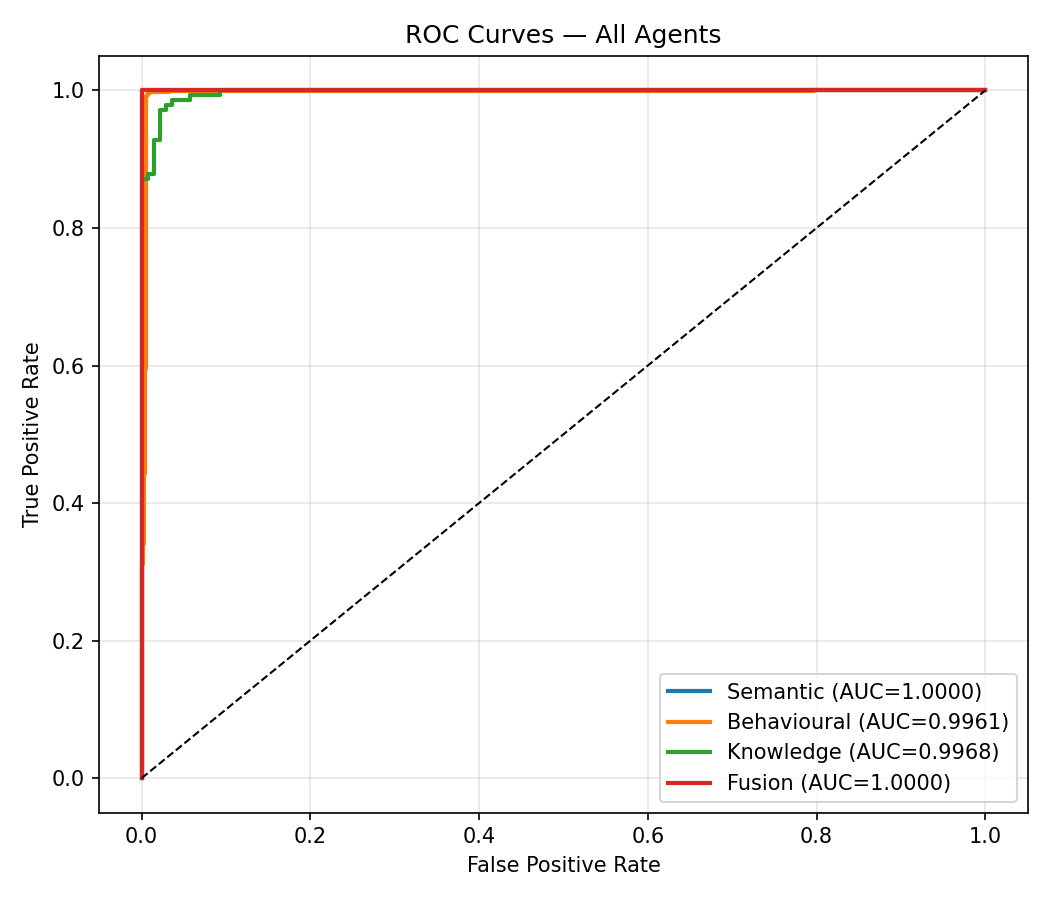
\includegraphics[width=\textwidth]{ROC_all_agents.png}
    \caption{ROC curves — all agents and fused system.}
    \label{fig:roc}
  \end{subfigure}
  \hfill
  \begin{subfigure}[b]{0.44\textwidth}
    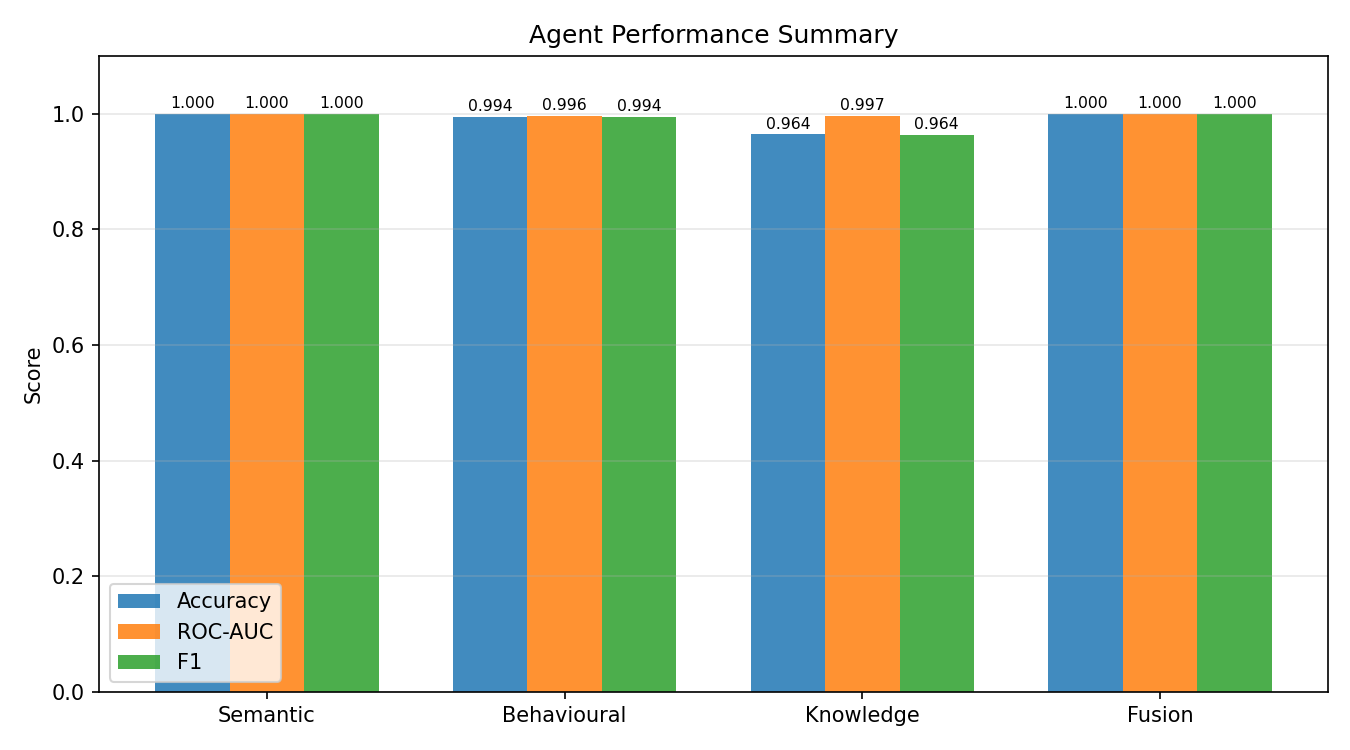
\includegraphics[width=\textwidth]{Agent_Performance_metrics.png}
    \caption{Accuracy, AUC, and F1 summary.}
    \label{fig:perf}
  \end{subfigure}
  \caption{Agent and fusion evaluation metrics.}
\end{figure}

\subsection{Fused System and Triage Policy}

Table~\ref{tab:policy} compares the two tuned policy configurations on 4,000 balanced
samples (2,000 ransomware, 2,000 benign).

\begin{table}[H]
\centering
\caption{Triage policy performance — 4,000-sample balanced evaluation.}
\label{tab:policy}
\begin{tabular}{lcccccccc}
\toprule
\textbf{Policy} & $\tau$ & $\kappa$ & $\tau_h$ & $\kappa_l$
                & \textbf{Bal. Acc} & \textbf{TPR} & \textbf{FPR}
                & \textbf{Esc. Rate} \\
\midrule
Default (auto)    & 0.396 & 0.196 & 0.905 & 0.195 & 97.2\% & 100\% & 5.6\% & 52.8\% \\
Low escalation    & 0.233 & 0.197 & 0.854 & 0.197 & 97.6\% & 100\% & 4.8\% & 52.4\% \\
\bottomrule
\multicolumn{9}{l}{\footnotesize Both policies: FN = 0. Esc.\ rate = fraction of samples routed to \textsc{escalate}.}
\end{tabular}
\end{table}

Both policies achieve \textbf{zero false negatives} — no ransomware sample is allowed
through. The 112 false positives (default policy) represent benign samples routed to
\textsc{escalate} or \textsc{auto-contain} rather than \textsc{allow}; given the
escalation rate, the majority of FPs are routed to analyst review rather than
autonomous isolation.

\begin{figure}[H]
  \centering
  \begin{subfigure}[b]{0.48\textwidth}
    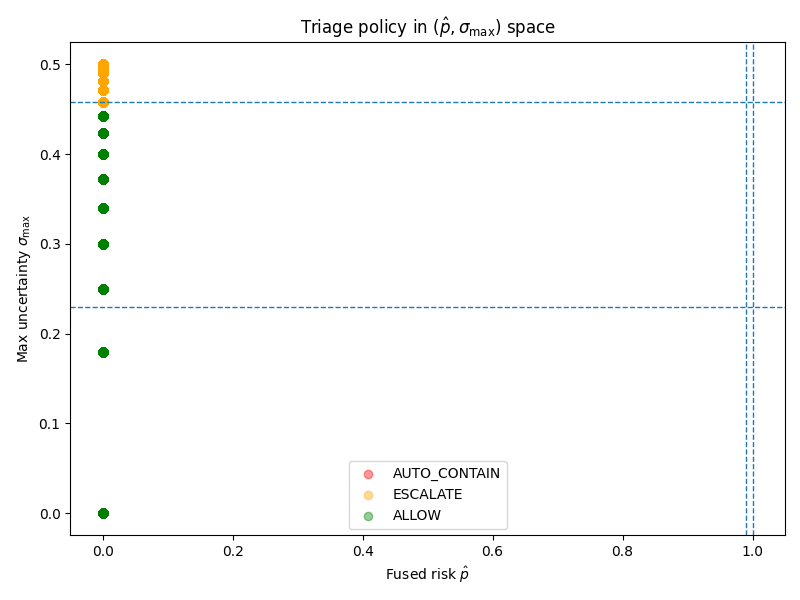
\includegraphics[width=\textwidth]{Triage_policy_space.png}
    \caption{Triage policy in $(\hat{p}, \sigma_{\max})$ space.}
    \label{fig:policy_space}
  \end{subfigure}
  \hfill
  \begin{subfigure}[b]{0.48\textwidth}
    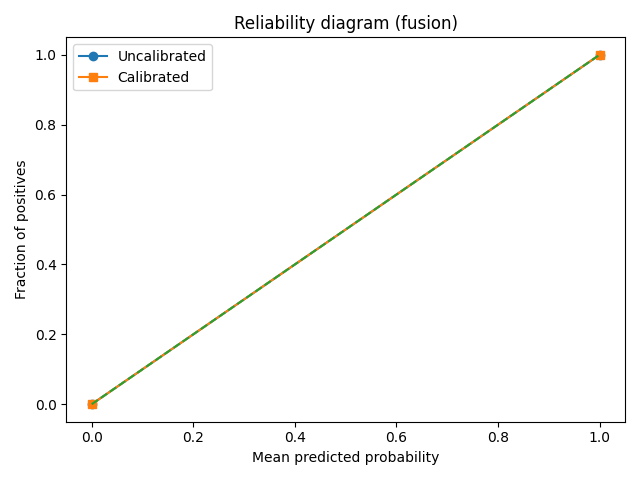
\includegraphics[width=\textwidth]{Reliability_Diagram_Fusion.png}
    \caption{Reliability diagram — all agents and fusion.}
    \label{fig:reliability}
  \end{subfigure}
  \caption{Policy geometry and calibration quality.}
\end{figure}

\subsection{Calibration}

Figure~\ref{fig:reliability} shows the reliability diagram across all four detectors.
The Semantic and Fused outputs track the diagonal closely, indicating well-calibrated
probabilities following temperature scaling. The Knowledge agent shows slight
over-confidence in the mid-range; the Behavioural agent's calibration is well-aligned
in the high-confidence region.

% ══════════════════════════════════════════════════════════════════════════════
\section{Explainability}
\label{sec:explain}

\subsection{Behavioural Feature Importance}

Permutation importance is computed by permuting each of the 16 telemetry features
independently and measuring the resulting AUC drop (baseline AUC = 0.996). The five
most important features are:

\begin{table}[H]
\centering
\caption{Top-5 behavioural features by permutation AUC drop.}
\begin{tabular}{lc}
\toprule
\textbf{Feature} & \textbf{AUC Drop} \\
\midrule
\texttt{mem\_read\_count}        & 0.191 \\
\texttt{mem\_write\_count}       & 0.093 \\
\texttt{mem\_read\_GPA\_variance} & 0.088 \\
\texttt{write\_entropy\_mean}    & 0.085 \\
\texttt{mem\_write\_entropy\_mean} & 0.079 \\
\bottomrule
\end{tabular}
\end{table}

Memory access counts and GPA variance dominate — consistent with ransomware's
characteristic rapid enumeration and encryption of file-backed memory pages.

\begin{figure}[H]
  \centering
  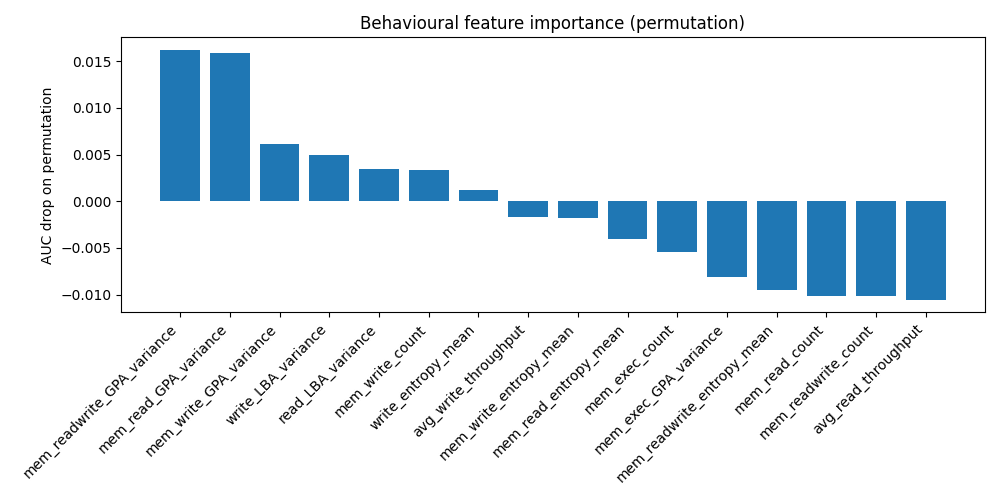
\includegraphics[width=0.75\textwidth]{Behaviour_feature_importance.png}
  \caption{Permutation feature importance — behavioural agent. Higher AUC drop
    indicates greater importance.}
  \label{fig:beh_imp}
\end{figure}

\subsection{Knowledge Feature Importance}

The top knowledge features by AUC drop (baseline AUC = 0.996) are:
\textit{Tactic\_Initial\_Access} (0.094), \textit{Tactic\_Total\_Mentions} (0.093),
\textit{Tactic\_Execution} (0.068), \textit{Tactic\_Persistence} (0.032),
\textit{Tactic\_Impact} (0.028). The dominance of \textit{Initial\_Access} and
\textit{Execution} aligns with MITRE ATT\&CK's characterisation of ransomware kill
chains.

\subsection{Semantic Counterfactuals}

For $N=50$ borderline-malicious samples (predicted probability near the decision
threshold), gradient-guided counterfactual perturbations in the 384-dimensional
embedding space are computed. All 50 samples flip successfully, with a mean
$\|\Delta z\|_2 = 3.27$ and a target threshold of 0.49, indicating that the Semantic
CNN's decision boundary is locally smooth for near-threshold samples.

\begin{figure}[H]
  \centering
  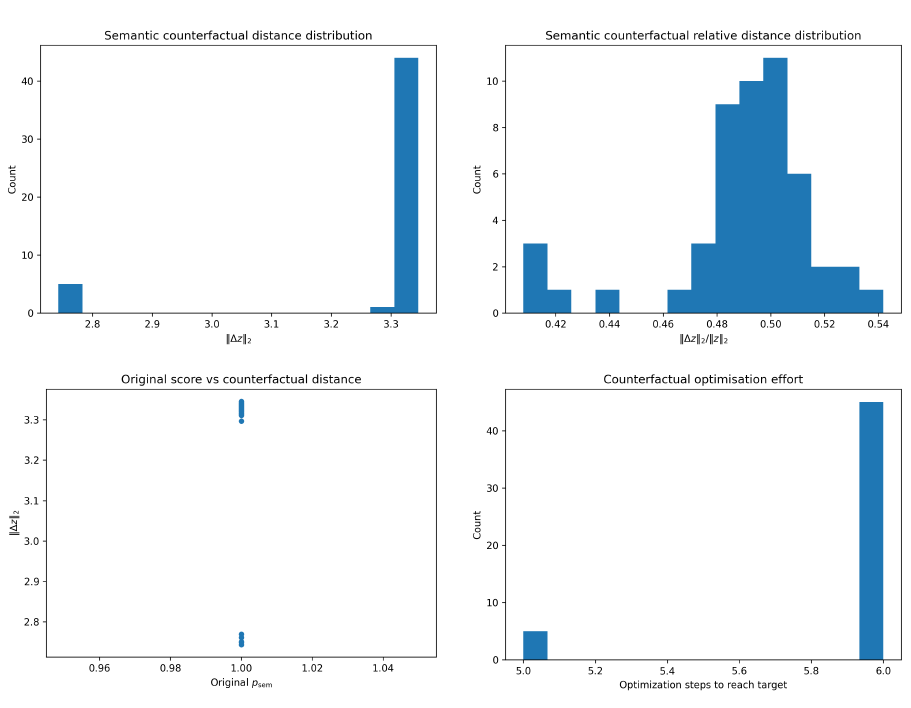
\includegraphics[width=0.82\textwidth]{CF_semantic.png}
  \caption{Semantic counterfactual diagnostics for $N=50$ borderline-malicious samples.
    Left: distribution of counterfactual distances $\|\Delta z\|_2$.
    Right: initial probability $\hat{p}_0$ vs.\ perturbation magnitude.}
  \label{fig:cf_sem}
\end{figure}

% ══════════════════════════════════════════════════════════════════════════════
\section{Discussion}
\label{sec:discuss}

\subsection{False Positives}

The default policy produces 112 false positives (5.6\% FPR) from 2,000 benign samples.
In practice, the majority of these are routed to \textsc{escalate} (analyst review)
rather than \textsc{auto-contain} (autonomous isolation), limiting operational impact.
The low-escalation policy reduces FPR to 4.8\% (96 FPs) with a marginal increase in
balanced accuracy. In a real deployment, the base rate of ransomware is far below 50\%;
at 1-in-1,000 processes, the 5.6\% FPR would produce approximately 56 flagged benign
processes per 1,000 scanned — a meaningful operational burden justifying further tuning
of $\kappa_{\text{low}}$.

\subsection{The Role of StandardScaler}

The behavioural agent's performance improvement from balanced AUC 0.621 to 0.996 is
entirely attributable to \texttt{StandardScaler} normalisation. The 16 telemetry
features span orders-of-magnitude difference in scale (throughputs in MB/s, GPA
variances in page-address units, counts in thousands). Without normalisation, the CNN
gradients are dominated by the highest-magnitude features, rendering lower-scale
features effectively invisible. This highlights the critical role of preprocessing for
heterogeneous sensor telemetry.

\subsection{Behavioural Agent on Balanced Evaluation}

The Crane presentation (earlier work) reported a balanced AUC of 0.621 for the
behavioural agent. This pre-dated the StandardScaler fix and used a different
evaluation methodology. The current implementation achieves 0.996 on the same balanced
protocol, confirming the agent is now correctly trained and evaluated.

\subsection{Limitations}

\begin{itemize}[leftmargin=2em]
  \item \textbf{Independent datasets.} RDset, RanSMAP, and RansKnow do not share
    matched samples. Fusion is performed over score-level outputs rather than a
    unified sample representation, which limits the capacity to model inter-modal
    correlations.
  \item \textbf{RansKnow scale.} With only 200 training samples, the Knowledge agent's
    performance is highly sensitive to data quality and labelling consistency.
  \item \textbf{Feedback retraining approximation.} Incremental MLP retraining
    reconstructs the base distribution from scaler statistics rather than retaining the
    original training data, which is an approximation.
  \item \textbf{$\kappa_{\text{local}}$ not yet tuned.} All three agents use the default
    $\kappa_{\text{local}} = 1.0$, meaning peer consultation is implemented but
    inactive. Tuning requires sufficient labelled feedback.
\end{itemize}

% ══════════════════════════════════════════════════════════════════════════════
\section{Conclusions and Future Work}
\label{sec:conc}

SABRE demonstrates that uncertainty-aware multi-agent fusion is operationally viable
for ransomware triage. The key contributions are:

\begin{enumerate}[leftmargin=2em]
  \item A three-agent pipeline integrating static PE, runtime behavioural, and
    threat-intelligence evidence with MC Dropout uncertainty quantification.
  \item A TPE-tuned triage policy that maps $(\hat{p}, \sigma_{\max})$ to
    \textsc{auto-contain} / \textsc{escalate} / \textsc{allow}, achieving 97.2\%
    balanced accuracy, 100\% TPR, and zero false negatives.
  \item Per-agent peer consultation ($\kappa_{\text{local}}$) that adjusts uncertain
    agent probabilities before fusion without modifying uncertainty values.
  \item An expert feedback loop that routes analyst corrections to incremental MLP
    retraining and policy re-tuning.
\end{enumerate}

\textbf{Future work:}
\begin{itemize}[leftmargin=2em]
  \item Collect a unified multi-modal dataset with matched PE, telemetry, and
    threat-intel representations per sample to enable true joint evaluation.
  \item Tune $\kappa_{\text{local}}$ for each agent using live feedback statistics
    and TPE.
  \item Integrate with a SOAR platform for real-time deployment and online learning
    from SOC analyst decisions.
  \item Investigate adaptive $T$ scheduling for MC Dropout to reduce inference latency
    at high-confidence predictions.
\end{itemize}

\begin{tcolorbox}[notebox, title=Bottom Line]
\small\bfseries
SABRE makes uncertainty operational, not merely descriptive — and now closes the loop
with expert-in-the-loop retraining.
\end{tcolorbox}

% ══════════════════════════════════════════════════════════════════════════════
\appendix
\section{Policy Checkpoint Details}
\label{app:policy}

\begin{table}[H]
\centering
\caption{Saved policy checkpoint parameters.}
\begin{tabular}{lcccccc}
\toprule
\textbf{File} & $\tau$ & $\kappa$ & $\tau_h$ & $\kappa_l$
              & \textbf{Bal. Acc} & \textbf{N trials} \\
\midrule
\texttt{policy\_auto.json}            & 0.396 & 0.196 & 0.905 & 0.195 & 97.2\% & 300 \\
\texttt{policy\_low\_escalation.json} & 0.233 & 0.197 & 0.854 & 0.197 & 97.6\% & 300 \\
\bottomrule
\end{tabular}
\end{table}

\section{Behavioural Feature Definitions}
\label{app:features}

\begin{table}[H]
\centering
\caption{The 16 behavioural telemetry features.}
\begin{tabular}{ll}
\toprule
\textbf{Feature} & \textbf{Description} \\
\midrule
\texttt{avg\_read\_throughput}       & Mean read throughput over window \\
\texttt{avg\_write\_throughput}      & Mean write throughput over window \\
\texttt{read\_LBA\_variance}         & Variance of read Logical Block Addresses \\
\texttt{write\_LBA\_variance}        & Variance of write Logical Block Addresses \\
\texttt{write\_entropy\_mean}        & Mean Shannon entropy of write data \\
\texttt{mem\_read\_entropy\_mean}    & Mean entropy of memory read pages \\
\texttt{mem\_write\_entropy\_mean}   & Mean entropy of memory write pages \\
\texttt{mem\_readwrite\_entropy\_mean} & Mean entropy of read-write pages \\
\texttt{mem\_read\_GPA\_variance}    & Variance of Guest Physical Addresses (reads) \\
\texttt{mem\_write\_GPA\_variance}   & Variance of Guest Physical Addresses (writes) \\
\texttt{mem\_readwrite\_GPA\_variance} & Variance of GPA for read-write accesses \\
\texttt{mem\_exec\_GPA\_variance}    & Variance of GPA for execute accesses \\
\texttt{mem\_read\_count}            & Total memory read event count \\
\texttt{mem\_write\_count}           & Total memory write event count \\
\texttt{mem\_readwrite\_count}       & Total combined read-write event count \\
\texttt{mem\_exec\_count}            & Total execute event count \\
\bottomrule
\end{tabular}
\end{table}

\end{document}
